\documentclass[a4paper,1pt]{report}
\usepackage[utf8]{inputenc}
\usepackage[spanish]{babel}
\usepackage{amsfonts}
\usepackage{amsthm}
\usepackage{amssymb}
\usepackage{amsmath}
\usepackage{graphicx}
\usepackage{subcaption}
\usepackage{float}
\usepackage[rightcaption]{sidecap}

\newtheorem*{pbo}{Principio del Buen Ordenamiento}

\newtheorem*{pim}{Principio de Inducción Matemática}

\newtheorem*{teo}{Teorema}

\newtheorem*{cor}{Corolario}

\newtheorem*{dem}{Demostración}

\newtheorem*{dfn}{Definición}

\newtheorem*{lem}{Lema}

\newtheorem*{prp}{Propiedades}


% Title Page
\title{Conferencia 5 - Planaridad}
\author{}

\begin{document}
\maketitle


\begin{dfn}
 Un grafo G es planar si existe un dibujo en el plano de G donde nunca dos de sus aristas se crucen.
\end{dfn}


\begin{figure}[H]
    \centering
    \begin{subfigure}[b]{0.45\textwidth}
    \centering
    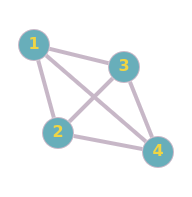
\includegraphics[width=0.4\textwidth]{figures5/G.png}
    \caption{G}
    \end{subfigure}
    \begin{subfigure}[b]{0.45\textwidth}
        \centering
    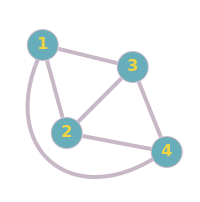
\includegraphics[width=0.4\textwidth]{figures5/Gplanar.png}
    \caption{Dibujo planar de G}
    \end{subfigure}
\end{figure} 

\begin{teo}
 Si G es planar entonces hay un dibujo de G que se puede hacer solo con líneas rectas
\end{teo}

\begin{figure}[H]
    \centering
    \begin{subfigure}[b]{0.45\textwidth}
    \centering
    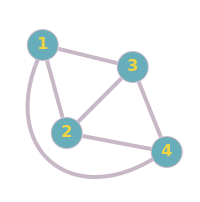
\includegraphics[width=0.4\textwidth]{figures5/Gplanar.png}
    \caption{Dibujo planar de G}
    \end{subfigure}
    \begin{subfigure}[b]{0.45\textwidth}
        \centering
    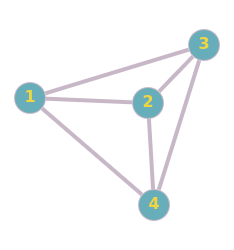
\includegraphics[width=0.4\textwidth]{figures5/Grectas.png}
    \caption{G con l\'ineas rectas}
    \end{subfigure}
\end{figure} 

\begin{dfn}
Una cara de un dibujo planar de un grafo planar es una región maximal del plano que no contiene ningún vértice o arista. 

\begin{figure}[H]
    \centering
    \begin{subfigure}[b]{0.45\textwidth}
    \centering
    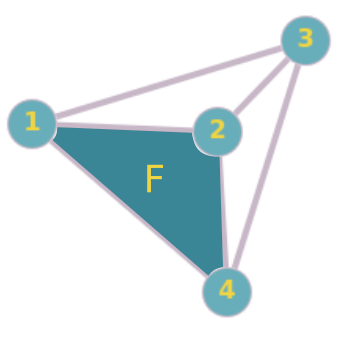
\includegraphics[width=0.4\textwidth]{figures5/face.png}
\end{subfigure}
\caption{F es una cara en el grafo G}
\end{figure} 

\begin{itemize}
 \item Toda cara interior está bordeada por un ciclo.
 \item Solo hay una cara externa.
\end{itemize}

\end{dfn}

\textbf{Nota:} Este tema se adentra en el campo de la Topología. En esta clase nos interesa más el dibujo del grafo y se
realizarán no se realizan las demostraciones de todos los teoremas por falta de formalismo en las cuestiones topológicas. (no son objetivo de la asignatura)\\


\textbf{Problema:} Dadas casas y servicios que se quieren brindar (agua, teléfono, electricidad, gas). Se desean
conectar casas con servicios sin que se crucen las conexiones de los servicios.


\begin{figure}[H]
    \centering
    \begin{subfigure}[b]{0.45\textwidth}
        \centering
        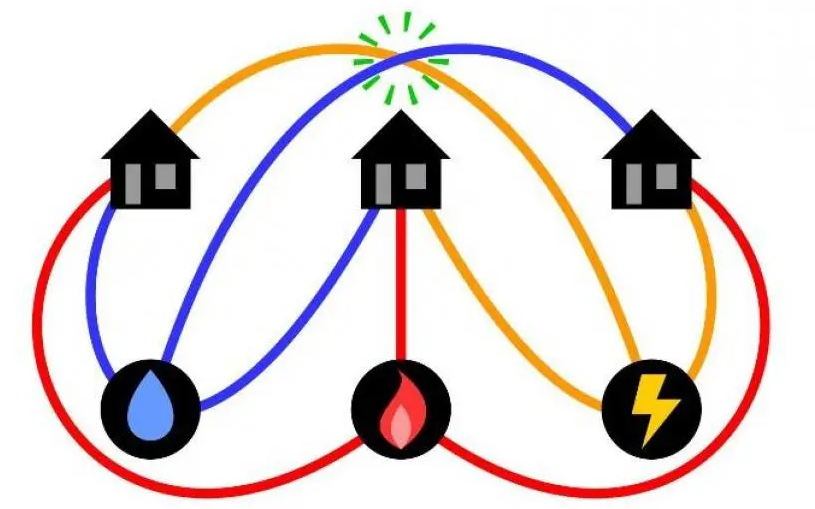
\includegraphics[width=\textwidth]{figures5/services.png}
    \end{subfigure}
\end{figure} 

Este problema en teoría de grafo sería: ¿Es posible pintar un grafo sin que se crucen sus aristas?


\textbf{Aplicaciones de la solución:} En toda rama donde se necesite aprovechar el espacio sin que los elementos se
solapen o entrecrucen. Por ejemplo, la nanotecnología, la fabricación de componentes electrónicas
(motherboards, chips).

\begin{teo}[Teorema de Euler]
Sea G un grafo conexo con $|E(G)|=m$  y $|V(G)|=n$, para todo dibujo planar de G se cumple que $n-m+f=2$ donde $f$ es la cantidad de caras del dibujo.
\end{teo}

Para la demostración del \textbf{Teorema de Euler} utilizaremos el siguiente lema:

\begin{lem}
 Si $m\geq n$ entonces G tiene al menos un ciclo.
\end{lem}

\begin{dem}
Demostremos el lema por el contrarrecíproco. 
\end{dem}

Sea G acíclico, entonces G se divide en componentes conexas $C_1,C_2,\dots,C_k$ donde para cada $C_i$ se tien que esta es conexa y acíclica, luego cada $C_i$ es un árbol por lo que $|E(C_i)|=|V(C_i)|-1$. 

Luego $m=|E(G)|=\sum^k_{i=1}|E(C_i)|=\sum^k_{i=1}|V(C_i)|-k=n-k$ y para $k=1$ se tiene entonces que $m\leq n-1 < n$\\

Ahora vamos a la demostración del Teorema.

\begin{dem}
Demostración del \textbf{Teorema de Euler} por inducción en el número de aristas
\end{dem}


\textbf{Caso base} Tomamos $m=n-1$ (mínima cantidad de aristas para que G sea conexo)

Como G es conexo y  $m=n-1$  entonces G es un \'arbol, luego es acíclico. Como G es acíclico entonces no tiene caras interiores, por tanto $f=1$ (tiene la cara exterior que es la única).

Por tanto, $n-m+f=n - (n-1)+1=2$\\



\textbf{Paso inductivo} Sea $m\geq n$.

Por el lema demostrado, en G existe al menos un ciclo, si se suprime una arista de dicho ciclo G no pierde conexidad y se obtiene G'  tal que \\
$|E(G$'$)| = m-1$ y $|V(G$'$)|=n$, además, como se pierde 1 ciclo también se pierde una cara, luego $n-(m-1)+ (f-1)=2$ y eso es $n-m+f=2$

\begin{dfn}
 El grado de una cara es la cantidad de aristas que participan en ella.
\end{dfn}


Nota: las aristas de corte se cuentan doble.

\begin{lem} \textbf{Faceshaking Lemma}
 Si un grafo planar G tiene k caras~($f_1,f_2,\dots,f_k$), entonces $\sum^k_{i=1}deg(f_i)=2|E(G)|$
\end{lem}

\begin{dem}
 
\end{dem}

\begin{itemize}
 \item El grado de una cara es el número de aristas que la bordean. En un grafo planar, cada arista limita dos caras exactamente.
 \item Luego, cada arista contribuye con 1 al grado de dos caras distintas.
 \item Por tanto, al sumar los grados de todas las caras, cada arista se cuenta exactamente dos veces. Entonces $\sum^k_{i=1}deg(f_i)=2|E(G)|$ $\blacksquare$.
\end{itemize}


\begin{dfn}
 Un grafo G es maximal planar si es planar y la adición de cualquier otra arista lo hace no planar
\end{dfn}

Nota: Todo grafo maximal planar es conexo

\begin{teo}
 Sea G un grafo conexo con $|V(G)|\geq 3$, G es maximal planar si y solo si toda cara de un dibujo planar es un triángulo, o sea,  dicha cara tiene grado 3
\end{teo}

\begin{dem}[$\Rightarrow$]
  G maximal planar $\Rightarrow$ Todas sus caras son de grado 3.
\end{dem}

Suponga que existe $c_i$ tal que $deg(c_i)\geq 4$. Luego, en $c_i$ hay al menos dos vértices que no son adyacentes, por tanto se puede trazar una arista entre ellos y no dejará de ser un dibujo planar. Y esto es una contradicción pues G es maximal planar.\\

\begin{dem}[$\Leftarrow$]
    Si G planar con todas las caras de grado 3 $\Rightarrow$ G maximal planar
\end{dem}

Supongamos que no es maximal, le podemos entonces agregar una arista $e$ al grafo sin romper la planaridad, sea $e = \{x,y\}$, quitando esa arista se tiene que $x, y$ son no adyacentes en G de donde la cara que los contiene tendr\'ia grado mayor o igual que 4. 

Luego G es maximal planar si y solo si toda cara de G tiene grado 3 $\blacksquare$

\begin{figure}[H]
    \centering
    \begin{subfigure}[b]{0.45\textwidth}
    \centering
    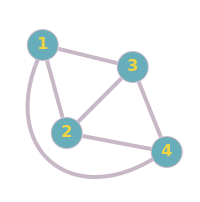
\includegraphics[width=0.5\textwidth]{figures5/Gplanar.png}
    \caption{G es maximal planar}
\end{subfigure}
\begin{subfigure}[b]{0.45\textwidth}
    \centering
    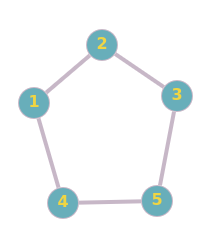
\includegraphics[width=0.4\textwidth]{figures5/C5.png}
    \caption{G no es maximal, si agregamos $\{2,4\}$ aun es planar}
\end{subfigure}
\end{figure} 

\begin{teo}
 Si G un grafo maximal planar donde $|E(G)|=m$  y $|V(G)|=n$ entonces $m=3n-6$
\end{teo}

\begin{dem}
 
\end{dem}

Si f es la cantidad de caras entonces $2m=3f$, por el Faceshaking Lemma, luego  
$f = \frac{2m}{3}$ y, por tanto, como $n-m+f=2$ entonces $n-m + \frac{2m}{3} = 2$ y despejando se tiene que $m=3n-6$


\begin{cor}
 Si G es planar entonces se cumple que $m\leq3n-6$
\end{cor}

\textbf{Demostración}

Si G no es maximal planar entonces se pueden añadir aristas hasta que lo sea, por tanto, 
$|E(G)|=m\leq3n-6$

\begin{lem}
 Si G es un grafo planar entonces G tiene al menos un vértice cuyo grado es menor o igual a 5
\end{lem}

\textbf{Demostración}

Suponga que no hay ningun vértice con grado menor que 5, luego para todo vértice $v$ de G se tiene que $deg(v)\geq 6$

luego se tiene entonces que $2m=\sum^n_{i=1} deg(v_i)\geq 6n$ y esto es contradicción pues $m\leq3n-6$\\

De manera similar se puede demostrar que tiene al menos 2 vértices con grado menor o igual a 5.

Similarmente, para al menos 4  vértices con grado menor o igual a 5.


\begin{dfn}
 Sea G un grafo y $e=\{x,y\}$ una arista de G. Una subdivisión de e consite en suprimir a esta y añadir un nuevo vértice z con las aristas $\{x,z\}$  y $\{z,y\}$. Si el grafo G se obtiene de un grafo H a través de una secuencia de subdivisiones de aristas de H. se dice que G es una subdivisión de H o que es homeomorfo con H.
\end{dfn}   

\begin{teo}[Teorema de Kuratowski]
 Un grafo G es planar si y solo si no contiene un subgrafo que sea una subdivisión de $K_5$ o de $K_{3,3}$
\end{teo}

\begin{dfn} 
Si un grafo G contiene una subdivisión de un grafo H como subgrafo, entonces decimos que H es un menor topológico de G. 
\end{dfn}

La operación contraria a la subdivisión es una contracción. Sin embargo, al contraer podemos eliminar cualquier vértice, no
solo un vértice de grado 2. Si hacemos eso, obtenemos lo que se llama un menor en el sentido más general.

\begin{teo}[Teorema de Wagner]
 Un grafo G es planar si y solo si no contiene a $K_5$ o  $K_{3,3}$  como menor (no necesariamente topológico). 
\end{teo}

Dado que un menor topológico es un menor en el sentido general, solo sería necesario probar que si un grafo contiene un menor de $K_5$ o  $K_{3,3}$, debe contener también un menor topológico de alguno de estos (no necesariamente el mismo).\\



\begin{figure}[H]
    \centering
    \begin{subfigure}[b]{0.45\textwidth}
        \centering
        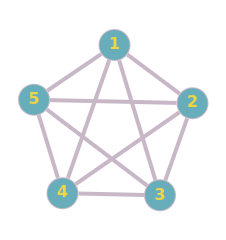
\includegraphics[width=0.45\textwidth]{figures5/K5.png}
        \caption{$K_5$}
    \end{subfigure}
    \begin{subfigure}[b]{0.45\textwidth}
        \centering
        \includegraphics[width=0.45\textwidth]{figures5/K33.png}
        \caption{$K_{3,3}$}
    \end{subfigure}
\end{figure} 

De manera general tanto \textbf{Kuratowski} como \textbf{Warner} expresan que para que un grafo  G sea planar no puede tener ``como parte de \'el'' ni a $K_5$ ni a $K_{3,3}$ 
\end{document} 
